% =====================================
% 【南京理工大学】 主题beamer模板
% 根据【中国科学院大学】主题的beamer模板进行定制
% 维护者:Shuai Qian (Andrew)
% 日期:2020/11/29
% 原始beamer主题地址:https://github.com/icgw/ucas-beamer
% =====================================

% 默认页面大小 4:3
\documentclass[10pt]{ctexbeamer}
% 页面大小 16:10
% \documentclass[10pt, aspectratio=1610]{ctexbeamer}
% 页面大小 16:9
% \documentclass[10pt, aspectratio=169]{ctexbeamer}
% 页面大小 14:9
% \documentclass[10pt, aspectratio=149]{ctexbeamer}
% 页面大小 1.41:1
% \documentclass[10pt, aspectratio=141]{ctexbeamer}
% 页面大小 5:4
% \documentclass[10pt, aspectratio=54]{ctexbeamer}
% 页面大小 3:2
% \documentclass[10pt, aspectratio=32]{ctexbeamer}

\usetheme[logo=NJUST]{ucas}


\title[Tilt-quadrotor]{南京理工大学}
\subtitle{beamer主题模板}
\author[Andrew]{\href{shuai.qian.anc@gmail.com}{Andrew}}
\institute{自动化学院 \\ {\small 南京理工大学}}
\date[\today]{\today}


\begin{document}

\begin{frame}[plain]
  \maketitle
\end{frame}

\begin{frame}[t]
  \frametitle{目录}
  \tableofcontents
\end{frame}

\section{1. PX4简介}\label{sec:1}
\begin{frame}
	\thispagestyle{empty}
	\begin{center}
		{\Large\bf \color{red} 1. PX4简介}
	\end{center}
\end{frame}

\subsection{开源飞控软件简介}

\begin{frame}[t]{开源飞行控制软件——PX4}
	\begin{block}{官网介绍}
		PX4 is an open source \textbf{flight control software} for drones and other unmanned vehicles. The project provides a flexible set of tools for drone developers to share technologies to create tailored solutions for drone applications. PX4 provides a standard to deliver drone \textbf{hardware} support and \textbf{software} stack, allowing an ecosystem to build and maintain hardware and software in a scalable way\footnote{https://px4.io/}.
	\end{block}
	
	\begin{itemize}
		\item 官网:https://px4.io/
		\item 代码管理:https://github.com/PX4/PX4-Autopilot
		\item 开发者手册:https://dev.px4.cc/master/zh/index.html
	\end{itemize}
\end{frame}

\begin{frame}[t]{PX4固件版本}
	\begin{itemize}
		\item 最新发布稳定版本\footnote{https://github.com/PX4/PX4-Autopilot/releases}:v1.11.2
		\item 使用版本:v1.10.0
	\end{itemize}
	\begin{figure}
		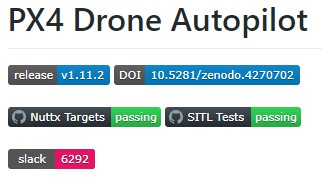
\includegraphics[scale=0.6]{image/release.jpg}
		\caption{PX4软件版本}
	\end{figure}
	不同版本的固件会修改一些bug、增加新的功能等。比如
	\begin{itemize}
		\item v1.10.0:多旋翼IMU数据更新速率1kHz
		\item v1.10.1:为了减小CPU的负载,将该速率降为400Hz
	\end{itemize}
\end{frame}


\subsection{PX4系统架构}

\begin{frame}[t]{PX4系统架构概述}
	PX4由两个主要部分构成:
	\begin{itemize}
		\item \textbf{飞行控制栈}(flight  stack):主要包括状态估计和飞行控制系统;
		\item \textbf{中间件}:该部分是一个通用的机器人应用层,可支持任意类型的自主机器人,主要负责机器人的内部/外部通讯和硬件整合。
	\end{itemize}
	
	所有的 PX4 支持的 无人机机型 (包括其他诸如无人船、无人车、无人水下航行器等平台)均共用同一个代码库。
	\begin{figure}
		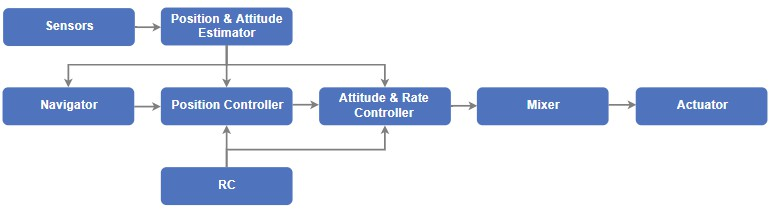
\includegraphics[scale=0.7]{image/stack.jpg}
		\caption{PX4飞行控制栈\footnote{https://dev.px4.io/master/zh/concept/architecture.html}}
	\end{figure}
\end{frame}



\section{2. 主要内容}\label{subsec:1-2}
\begin{frame}
	\thispagestyle{empty}
	\begin{center}
		{\Large\bf \color{red} 2. 主要内容}
	\end{center}
\end{frame}


\begin{frame}[t]{文本区块}
  将文本放入区块内
  
  \begin{block}{普通区块}
    这是普通色块
  \end{block}

  \begin{exampleblock}{示例区块}
    \red{红色}
  \end{exampleblock}

  \begin{alertblock}{强调区块}
    \green{绿色}
  \end{alertblock}

\end{frame}


\section{3. 总结}\label{subsec:1-3}
\begin{frame}
	\thispagestyle{empty}
	\begin{center}
		{\Large\bf \color{red} 3. 总结}
	\end{center}
\end{frame}



\begin{frame}[t]{引用}
  \begin{theorem}\label{thm1}
    \[\textbf{具体 (\red{Concrete})} = \textbf{连续 (\red{Con}tinuous)} + \textbf{离散 (Dis\red{crete})}\]
  \end{theorem}
  \vfill
  \begin{proof}
  	比如证明过程中需要插入公式:
    \begin{equation}\label{equation-1}
    \alpha = \beta + \gamma
    \end{equation}
  \end{proof}
  这里还可以引用定理~\ref{thm1}.
\end{frame}


\begin{frame}[t]{自定义字体大小}
  \begin{center}
    \begin{tabular}{ll}
      \Huge  $\backslash$Huge                & \Huge \structure{24.88 pt}     \\
      \huge  $\backslash$huge                & \huge \structure{20.74 pt}     \\
      \LARGE $\backslash$LARGE               & \LARGE \structure{17.28 pt}    \\
      \Large $\backslash$Large               & \Large \structure{14.4 pt}     \\
      \large $\backslash$large               & \large \structure{12 pt}       \\
      \normalsize $\backslash$normalsize     & \normalsize \structure{10 pt}  \\
      \small $\backslash$small               & \small \structure{9 pt}        \\
      \footnotesize $\backslash$footnotesize & \footnotesize \structure{8 pt} \\
      \scriptsize $\backslash$scriptsize     & \scriptsize \structure{7 pt}   \\
      \tiny $\backslash$tiny                 & \tiny \structure{5 pt}
    \end{tabular}
  \end{center}
\end{frame}
\makeatother


\begin{frame}[plain]
  \vfill
  \centerline{\huge 谢谢}
  \vfill
\end{frame}

\end{document}
